\documentclass{article}

\usepackage[a4paper]{geometry} 
\usepackage[dutch]{babel} % Juiste afbreekregels en dergelijke!
\usepackage{parskip} % Alinea's beginnen links uitgelijnd en er staat een lege regel tussen alinea's.
\usepackage{amsmath, amssymb, textcomp} % Wiskundige symbolen e.d.
\usepackage{color} % Kleuren
\usepackage{graphicx} % Plaatjes
\usepackage{enumerate} % Voor opsommingen
\usepackage[official]{eurosym}
\usepackage{url} % Voor het weergeven van hyperlinks
\usepackage{float}
%\usepackage{minted} % Voor source-code weergeven
\usepackage{gensymb}
\usepackage[hidelinks]{hyperref} % Voor clickable links van refs
\usepackage[nottoc,numbib]{tocbibind} % Om de referenties in de inhoudsopgave te krijgen

\setcounter{secnumdepth}{0} % Om ervoor te zorgen dat er geen hoofdstuknummers voor de hoofdstuktitels komen

\title{Testverslag ATP\\
		   Lemonator}
\author{Philippe Zwietering\\
	           Studentnummer: 1685431}
           
\begin{document}
	\maketitle
      	
    \clearpage
    
    \section{Inleiding}
    
    In dit document wordt besproken welke tests zijn uitgevoerd voor het ATP lemonator project en welke kwaliteit die hadden om de zekerheid van dit project te waarborgen. Het beschrijft ook in welke mate er is afgeweken van het testplan.
    
    \section{Gebruikte infrastructuur} 
    Tijdens het project is gebruik gemaakt van bepaalde tools voor het automatiseren en analyseren van de tests en van tools voor het algemeen bevorderen van het projectverloop.
    
    \subsection{Tools}
    Voor dit project is gebruikgemaakt van git als versiebeheer met GitHub als serverplatform. Op die manier kon enigszins zeker worden gesteld dat alle versies correct worden beheerd op een externe server, ook al heb ik dit project in mijn eentje uitgevoerd. 
    
    Dit project is voornamelijk geschreven in Python 3.7 en op een gegeven moment is er ook gebruikgemaakt van C++ 11+ voor het schrijven van de C++ Controller. Het project is geschreven op een 64-bits Linux systeem. Om de simulaties uit te voeren moet in de command line python3 main.py worden uitgevoerd, met als optionele argumenten --py en --cpp, respectievelijk voor de Python controller en de CPP controller. Als er geen argument wordt gekozen, wordt automatisch de Python controller gebruikt.
    
    Om tests uit te voeren is gebruikgemaakt van het nose2 package van Python. nose2 maakt gebruik van het unittest package, wat een vrij standaard manier is om tests op te stellen. nose2 kan automatisch alle tests in een map zoeken en uitvoeren, met ondersteunende functionaliteit voor setUps zodat bepaalde code opgezet kan worden voor alle tests van dezelfde smaak zodat dit niet iedere keer opnieuw hoeft worden geschreven. Om dit uit te voeren typt men nose2 in de betreffende map. Het enige waar voor gezorgd moet worden is dat alle testklasses en functies beginnen met test, de rest gebeurt vanzelf.
    
    Om de coverage van de Pythontests te meten wordt gebruikgemaakt van de coverage module van Python. Deze kan rapporten genereren voor de coverage van de tests, zodat kan worden gecheckt dat ten minste alle code afgegaan wordt in de hoop dat alle aspecten van de code ook getest wordt. Om een coverage report te geven van de tests van nose2 kan nose2 --with-coverage worden uitgevoerd op de command line in de relevante map.
    
    Verder wordt er voor het C++ gedeelte van de opdracht gebruikgemaakt van Pybind11 en cppimport, een Python module die het makkelijker maakt om pybind11 te gebruiken. Dit scheelt enorm veel werk en gedoe met buildfiles en CMake. Het is voor het builden van dit project dus nodig dat de volgende modules en libraries van tevoren goed worden ge\"installeerd: coverage, nose2, unittest, cppimport en als C++-dependency pybind11.
    
    \subsection{Mappenstructuur}
    Uiteindelijk is voor dit project alleen de simulatormap gebruikt. Ik weet dat dit niet netjes is, maar wegens tijdgebrek en wegens gemakzucht heb ik ervoor gekozen om alle Python code in dezelfde map te zetten, zodat ik niet moeilijk hoefde te doen met de sys.path, wat me aardig wat hoofdpijn bezorgde in het begin van dit project. Ook de C++-controller staat in deze map, zodat makkelijk ge\"importeerd en ge\"exporteerd kan worden. Al deze code staat in de simulator map, de overige mappen worden door de student niet gebruikt.
    
    \section{Reproduceerbaarheid tests}
    Voor de tests wordt dus gebruikgemaakt van nose2 en unittest. Het unittesten gebeurt hierdoor op een gestandaardiseerde manier, en sommige integration tests die niet handmatig moeten worden gecontroleerd kunnen op een gelijkwaardige manier gebeuren. De unittests en system integration tests zijn namelijk allemaal op dezelfde manier opgebouwd: ze vallen in een bepaalde TestCase klasse die alle mogelijke functies hoort af te gaan voor een bepaalde klasse van de code. In de setUp functie van de TestCase klasse wordt alle code geschreven die alle tests nodig hebben van die klasse. Zie de afbeelding voor een voorbeeld. Deze setUp code wordt voor iedere testfunctie opnieuw uitgevoerd, dus er is geen onderline afhankelijkheid. Zoals ook te zien is wordt er getest door middel van asserts: faalt deze dan faalt de test. Dit wordt gebruikt om variabelen langs te gaan die relevant worden geacht voor de unittest en te checken of die de waarden hebben die ze zouden moeten hebben.
    
    Om de tests uit te voeren kan nose2 worden uitgevoerd in de command line in de simulator map. Alle tests die zijn geschreven met behulp van unittest worden dan langsgegaan. Voor een coverage report kan nose2 --with-coverage uit worden gevoerd. Om vervolgens per bestand een uitgebreid report te krijgen kan coverage html -i worden uitgevoerd, dit geeft in de htmlcov map dan een uitgebreid overzicht van de coverage per bestand.
    
    \begin{figure}[H]
    	\centering
    	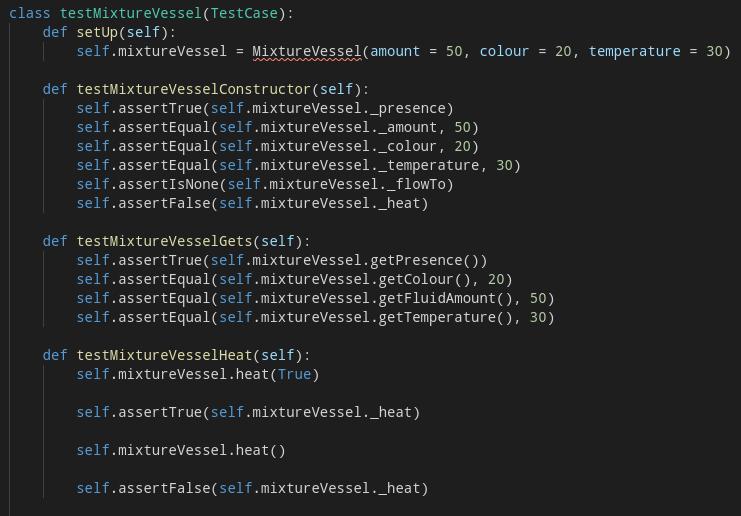
\includegraphics[width=0.9\textwidth]{figures/setup.png}
    	\caption{Voorbeeld unittest (er zijn er nog meer voor deze klasse)}
    \end{figure}

	\section{Test verantwoording}
	Er zijn voor dit project zowel whitebox unittests als whitebox system integration tests voor de controllers geschreven. 
	Qua unittests zijn er voornamelijk 2 typen tests: een bestand checkt via mocks de SimulatorProxy en een bestand checkt alle functionaliteit van de plant van de simulator. De SimulatorProxy wordt dus alleen gecheckt op het uitvoeren van de corresponderende functies van de plant, omdat de functionaliteit alleen maar gecheckt hoeft te worden bij de daadwerkelijke simulatie. Wel is de SimulatorProxy uiteindelijk gebruikt voor het maken van de simulators. Het is vrij belangrijk om unittests uit te voeren voor de plant, omdat dan kan worden gecontroleerd dat fouten in de Controller niet toevallig veroorzaakt worden door een waarde die verkeerd wordt uitgelezen of doorgegeven. De controller is ook volledig doorgelicht met behulp van system integration tests. Iedere van de Python controller en alle verschillende programmatakken zijn gecovered. De coverage van de CPP controller kan niet worden gecheckt, maar omdat exact dezelfde tests voor de Python en CPP controllers worden gebruikt, is het aannemelijk dat ook de CPP controller voldoende gecovered is.
	
	In totaal worden er 120 tests uitgevoerd door nose2 van in totaal een slordige 1400 regels code als de dubbele controller tests voor Python en CPP niet worden meegerekend. Hiervan zijn de system integration tests aanzienlijk groter en uitgebreider dan de unittests. Naast deze tests zijn er geregeld smoke tests uitgevoerd voor de simulatie zelf, om code te checken en aanpassingen te maken. Dit is echter niet op een gestructureerde manier gegaan, en was meer om de tests zelf ook af en toe te controleren. 
	
	Voor de unittests zijn de volgende dingen getest:
	\begin{itemize}
		\item Abstract Interface: voor iedere effector en sensor van de plant is een interface gemaakt zodat de hele simulatie de plant via proxy kan aanroepen. Het aanroepen is getest via mocks.
		\item Vessel: alle functionaliteit voor normale vessels, dus constructor, de getters, flow met meerdere klassen initi\"ele waarden en meerdere soorten vessels waarnaartoe wordt geflowd en wat er gebeurt met kleur.
		\item MixtureVessel: alle extra functionaliteit voor MixtureVessels bovenop normale Vessels, dus alle relevante dingen die kunnen gebeuren bij de update, presence en heater.
		\item Effector: alle basisfunctionaliteit voor de effectoren. Dit zijn dus de constructor en het aan- en uitzetten.
		\item Pump: de extra functionaliteit bovenop effector, dus het drukzetten en laten afnemen en laten vloeien van vloeistoffen.
		\item Valve: praktisch het enige extra wat valves doen is het equaliseren van de druk in de pompen, dit is hier getest.
		\item Heater: controleren dat de heater daadwerkelijk de temperatuur verhoogt in een vessel.
		\item LED: het togglen van ledjes en de extra getter voor kleur.
		\item LCD: tabs lijken niet te werken en ik kreeg ze met geen mogelijkheid werkend. Verder, verificatie van getLines, pushString, clear en put.
		\item Sensor: alles basisfunctionaliteit voor sensoren. Dit zijn dus de constructor, het lezen en meten van waarden en het omzetten van de waarde naar de natuurkundige waarde die daadwerkelijk iets voorstelt.
		\item ColourSensor: testen dat kleuren goed gemeten worden.
		\item TemperatureSensor: testen dat de temperatuur goed omgezet wordt.
		\item LevelSensor: testen dat het vloeistofniveau goed wordt omgezet.
		\item PresenceSensor: testen dat deze sensor goed omgaat met afwezigheid van een vessel.
		\item Keypad: controleren dat de toetsen goed in de FIFO worden gezet en er ook weer goed uitkomen.
	\end{itemize}

	Voor de system integration tests zijn alle mogelijke inputs in de verschillende stadia afgegaan en gekeken of de output correspondeert met de gewenste output. Dit lijkt zo te zijn. Er is uiteindelijk een coverage van 96\% gehaald, maar hier is de coverage van de CPPController dus niet meegenomen en ook niet de de coverage van de plant, omdat die niet kunnen worden gecheckt door de coverage tool omdat dit binaire bestanden zijn. Echter heb ik mijn uiterste best gedaan om alle states van alle functies af te gaan en ook foute invoer te testen. Daarnaast is de coverage niet hoger omdat de main.py en de abstracte interface niet volledig worden afgegaan. De main.py omdat die simpelweg niet getest hoeft te worden en de abstracte proxy-interface omdat hij de error handling daar als regels telt, waarvan je juist wilt dat die niet afgegaan worden, want dat betekent dat je een fout hebt gemaakt.
	
	\section{Afwijkingen van het testplan}
	In het testplan had ik een aantal dingen genoemd waaraan voldaan zouden moeten worden. Uiteindelijk heb ik niet alles gehaald. Ik heb in overleg met de opdrachtgever geen enkel aspect uitgevoerd dat te maken heeft met de hardware van de lemonator. Ook heb ik uiteindelijk geen blackbox testing gedaan, maar dit vervangen met whitebox testing. Dit leek me beter, omdat er dan makkelijker automatisch getest kan worden en het concreter is wat er precies fout gaat in het programma. Verder heb ik voldaan aan mijn testplan.
    
\end{document}}